\documentclass[11pt]{article}
\usepackage[spanish]{babel}
\decimalpoint
\usepackage[utf8x]{inputenc}
\usepackage{amsfonts}
\usepackage{MnSymbol}
\usepackage{graphicx}
\usepackage{float}
\usepackage{wasysym}
\usepackage{pdfpages}
\usepackage[margin=0.5in,left=1in,right=1in, bottom = 1in, includehead]{geometry}
\usepackage{amsmath}
\usepackage{multicol}
\usepackage{caption}
\usepackage{subcaption}
\renewcommand{\baselinestretch}{1.3}
\usepackage{booktabs}
\usepackage{soul}

%% NEW Commands
\newcommand{\klein}{\text{*}}  
\newcommand{\R}{\mathbb{R}}
\newcommand{\N}{\mathbb{N}}

\newcommand{\red}[1]{\textcolor{red}{#1}}
\newcommand{\blue}[1]{\textcolor{blue}{#1}}
\newcommand{\green}[1]{\textcolor{green}{#1}}


\title{Reporte semanal: Agosto 25-Septiembre 14 \textcolor{red}{\st{Agosto 31}}} 
\author{Jorge Ballote}
\begin{document}

% \includepdf[pages=1]{portada_proyecto_02.pdf}
\maketitle
% ---- 1. INTRODUCCIÓN -----------------------------------------
\section{Introducción} A continuación se presenta el reporte de resultados de la tercera semana.

% ---- 2. Objetivos de la semana -----------------------------------------
\section{Objetivos de la semana}
Esta semana fue destinada a lo siguiente.
\begin{enumerate}
    \item Algoritmo genético para la optimización de hiper parámetros.
    \item Transformaciones a las series de tiempo para la investigación de diferentes patrones
\end{enumerate}
Los objetivos fueron cumplidos. En las siguiente secciones, se analizan los resultados obtenidos.

% ---- 3. ALGORITMOS -----------------------------------------
\section{Modificaciones al algoritmo}
Se implementó una modificación al algoritmo inicial para transfomar las traces con funciones trigonométricas. Además, se implementó un algoritmo genético para optimizar hiperparámetros.

\subsection{Transformaciones de series de tiempo}
En el artículo se describe que se han obtenido buenos resultados, transformando las series de tiempo con funciones trigonométricas. La lógica detrás de esto, consiste en que al aplicar una transformación, las traces lucirán muy diferentes a las originales, y en teoría nuestra grid debería ser capaz de detectar patrones nuevos con estas nuevas traces.

\begin{figure}[H]

    \centering
    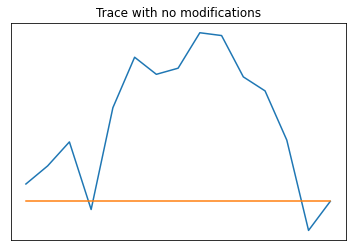
\includegraphics[width=.3\textwidth]{../src/imgs/trace.png}\hfill
    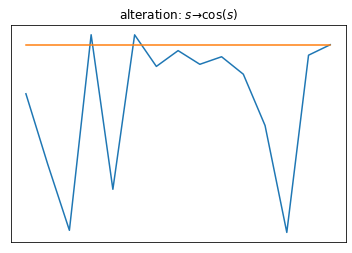
\includegraphics[width=.3\textwidth]{../src/imgs/trace_cos.png}\hfill
    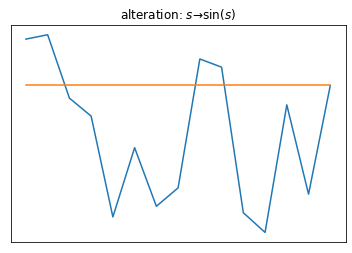
\includegraphics[width=.3\textwidth]{../src/imgs/trace_sin.png}
    
    \caption{Diferencias entre traces con diferentes operadores aplicados.}
    \label{fig:figure3}
    
\end{figure}

Una pregunta importante es, ¿Se aplica la función trigonométrica a cada trace o a los precios en el tiempo?

Supongamos que tenemos una serie de tiempo $a_1, ..., a_n$ y un valor siguiente $a_{n+1}$. Las traces se obtienen normalizando con el punto final. Es decir 
\begin{equation}
    b_i = \frac{a_i}{a_n}-1. 
\end{equation}
De modo que siempre ocurre que $b_n = \frac{a_n}{a_n} -1 = 0$. Esta es una propiedad que nos gustaría preservar. Por otro lado, para saber si estamos en presencia de una trace ganadora o perdedora, lo que se hace es sencillamente comparar si $a_{n+1} > a_n$ o biseversa. Llamaremos label entonces al siguiente valor:
\begin{equation}
    label = \frac{a_{n+1}}{a_n} -1
\end{equation}
También es importante que nuestra label se preserve usando los valores sin modificar (Es decir, antes de aplicar algún operador a la serie de tiempo). De modo que dado un operador $f: \mathbb R \to \mathbb R$, nuestra trace modificada esta dada por
\begin{equation}
    c_i = \frac{f(a_i)}{f(a_n)}-1, \quad label = \frac{a_{n+1}}{a_n} -1.
\end{equation}
Las funciones implementadas fueron, $\sin, \cos$ y $\tan$.  Los resultados se presentaran en la siguente sección, después de haber sido optimizados con nuestro algoritmo genético

\subsection{Optimización de hiperparámetros con un algoritmo genético}
\subsubsection{Introducción a algoritos genéticos}
Describiremos brevemente lo que es un algoritmo genético, para más información, consultar a [2].

El algoritmo implementado, está inspirado en el proceso natural de la evolución. Nuestro conjunto de hiperparámetros por optimizar se conocen como cromosomas en este contexto. Y cada hiperparámetro es un gen.

Se tiene una población de soluciones inicial conocida como generación 0. A partir de ahí, usamos los elementos de cada generación para crear a la siguente. Los genes tienen más posibilidades de preservarse conforme mejor resultados proporcionen, es decir, mientras más valor tenga una Fitness function. Usualmente se usa la accuracy, pero en nuestro caso usaremos criteria2 = $\min(5p,1)(2a-1)$.

Para dar lugar a la evolución es necesario el operador \textsl{crossover} que combina genes de dos miembros de la población, para obtener un nuevo cromosoma. Además de eso, se procura la diversidad de soluciones, utilizado un operador de mutación, que puede seleccionar una solución y modificarla ligeramente (Cambiarle un parámetro en nuestro caso).  

En algunas ocasiones, se implementa el concepto de elitismo, que consiste en forzar a las mejores soluciones a permanecer siempre en la población.

% ---- 4. Metodología -----------------------------------------
\section{Metodología}
Corrimos nuestro algoritmo genético durante 20 generaciones por experimento. Con una población de tamaño 30. La probabilidad de crossover fue seleccionada de 0.9 y la de mutación de 0.5. Se utilizó un algoritmo elitista, donde las 5 mejores soluciones permanecían siempre como miembros de la población. Tal como se describió, la métrica que nos interesa es $\min(5p,1)(2a-1)$, de modo que esa será la métrica a optimizar en nuestro algoritmo genético. En particular, tomando $p:$ 'part above' y $a:$ 'acc above'

Para la presentación de resultados, usaremos 2 formas de evaluar nuestro algoritmo. 
\begin{enumerate}
    \item \textbf{Desempeño en los últimos días:} Simplemente, ¿Si hubiésemos usado nuestro algoritmo en los últimos $d$ días, ¿Cuántas veces hubiésemos acertado?
    \item \textbf{K-Cross Validation} El k-cross validation consiste en particionar nuestro conjunto de datos en $K$ partes diferentes. De modo que entrenamos $k$ veces nuestro modelo, utilizando $k-1$ conjuntos de la partición para el entrenamiento y  el conjunto restante para la validación. Finalemente, se suele tomar la media de los $k$ resultados obtenidos
\end{enumerate}

Para la optimización de hiperparámetros se utilizaron $n-365$. Para la prueba del modelo, se utilizaron $365$ días de nuestro vector de precios. Cada posible cromosoma de nuestro algoritmo, indujo un conjunto de traces, los cuales fueron utilizados para conseguir la puntuación del $k$-cross validation con $k=4$.

Las métricas a consideran serán las utilizadas en el reporte previo. Incluyendo el criterio 2.

\section{Resultados}
Después de 25 generaciones, nuestra Fitness function alcanzó un valor máximo de 0.16403. Al hacer la prueba de los últimos 365 días se obtienen muy buenos resultados, lo cuál sugiere que los parametros obtenidos son capaces de generalizar.
\begin{table}[H]
    \centering
    \begin{tabular}{|ll|}
        \hline
        \multicolumn{2}{|c|}{Hiperparámetros} \\
        \hline
        trace\_size            &           95 \\
        height                &           20 \\
        width                 &           95 \\
        grid\_type             &         wins \\
        operation\_type        &          W/L \\
        alpha\_plus            &     0.825204 \\
        alpha\_minus           &     0.686667 \\
        eliminate\_noise\_thold &  0.000251377 \\
        \hline
        \end{tabular}
    $\Rightarrow$
    \begin{tabular}{|ll|}
        \hline
        \multicolumn{2}{|c|}{Resultados}\\
        \hline
        \textbf{criteria2\_above}            &        \textbf{0.232} \\
        accuracy            &         53.75 \\
        participation                &          47.39 \\
        acc\_above                 &         61.60 \\
        part\_above             &       30.68 \\
        acc\_below        &        39.34 \\
        part\_below            &   16.71 \\
        \hline
        \end{tabular}
\end{table}



\subsection{Alteración: $s \to \sin(s)$}

\begin{table}[H]
    \centering
    \begin{tabular}{|ll|}
        \hline
        \multicolumn{2}{|c|}{Hiperparámetros} \\
        \hline
        trace\_size            &          79 \\
        height                &           4 \\
        width                 &          79 \\
        grid\_type             &        wins \\
        operation\_type        &         W/L \\
        alpha\_plus            &  0.00423783 \\
        alpha\_minus           &    0.131058 \\
        eliminate\_noise\_thold &   0.0091428 \\
        \hline
        \end{tabular}
    $\Rightarrow$
    \begin{tabular}{|ll|}
        \hline
        \multicolumn{2}{|c|}{Resultados}\\
        \hline
        \textbf{criteria2\_above} & \textbf{0.219} \\
        accuracy            &         50.70 \\
        participation                &          96.71 \\
        acc\_above                 &         60.97 \\
        part\_above             &       44.93 \\
        acc\_below        &        41.79 \\
        part\_below            &    51.78 \\
        \hline
        \end{tabular}
\end{table}
En el proceso de entrenamiento, obtuvo en promedio \texttt{criteria2 = 0.123}. En la prueba de los últimos 365 días, se obtuvo que  \texttt{criteria2 = 0.219}.

\subsection{Alteración: $s \to \cos(s)$}
\begin{table}[H]
    \centering
    \begin{tabular}{|ll|}
        \hline
        \multicolumn{2}{|c|}{Hiperparámetros} \\
        \hline
        trace\_size            &         97 \\
        height                &         52 \\
        width                 &         97 \\
        grid\_type             &   earnings \\
        operation\_type        &        W/T \\
        alpha\_plus            &   0.171751 \\
        alpha\_minus           &  0.0240919 \\
        eliminate\_noise\_thold &  0.0394345 \\
        \hline
        \end{tabular}
    $\Rightarrow$
    \begin{tabular}{|ll|}
        \hline
        \multicolumn{2}{|c|}{Resultados}\\
        \hline
        \textbf{criteria2\_above} & \textbf{0.133} \\
        accuracy            &         50.99 \\
        participation                &          96.71 \\
        acc\_above                 &         56.69 \\
        part\_above             &       69.58 \\
        acc\_below        &        36.36 \\
        part\_below            &     27.12 \\
        \hline
    \end{tabular}
\end{table}

En el proceso de entrenamiento, obtuvo en promedio \texttt{criteria2\_above = 0.123}. En la prueba de los últimos 365 días, se obtuvo que  \texttt{criteria2\_above = 0.133}.
\subsection{Alteración: $s \to \tan(s)$}
\begin{table}[H]
    \centering
    \begin{tabular}{|ll|}
        \hline
        \multicolumn{2}{|c|}{Hiperparámetros} \\
        \hline
        trace\_size            &         45 \\
        height                &         95 \\
        width                 &         45 \\
        grid\_type             &       wins \\
        operation\_type        &        W/L \\
        alpha\_plus            &  0.0358503 \\
        alpha\_minus           &   0.103658 \\
        eliminate\_noise\_thold &  0.0391943 \\
        \hline
        \end{tabular}
    $\Rightarrow$
    \begin{tabular}{|ll|}
        \hline
        \multicolumn{2}{|c|}{Resultados}\\
        \hline
        \textbf{criteria2\_above} & \textbf{0.133} \\
        accuracy            &          50.86 \\
        participation                &         95.34 \\
        acc\_above                 &          56.66 \\
        part\_above             &       65.75 \\
        acc\_below        &        37.96 \\
        part\_below            &    29.58 \\
        \hline
    \end{tabular}
\end{table}
\dotfill
\begin{figure}[H]
    \centering
    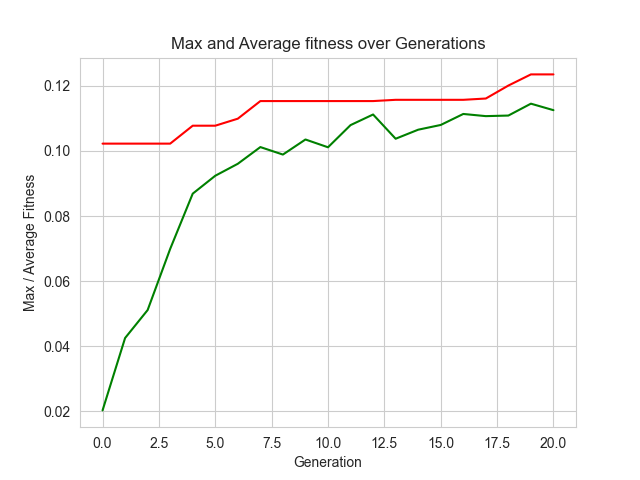
\includegraphics[width=.45\textwidth]{../src/imgs/genetic_sin.png}
    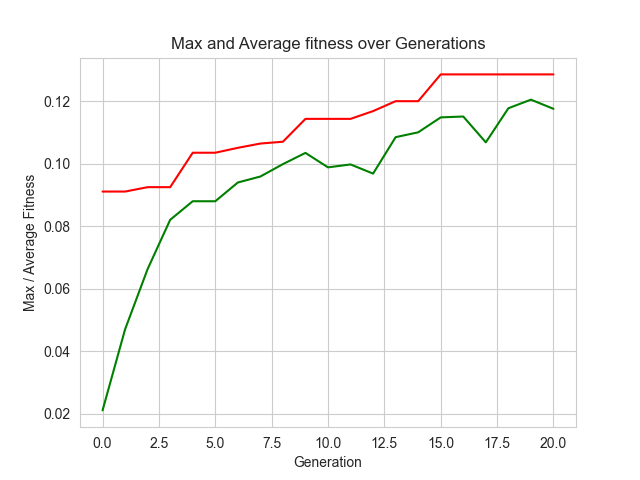
\includegraphics[width=.45\textwidth]{../src/imgs/genetic_cos.png}
    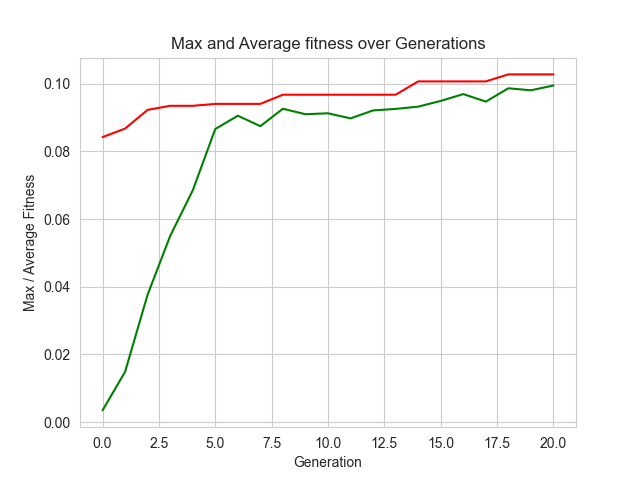
\includegraphics[width=.45\textwidth]{../src/imgs/genetic_tan.png}
    \caption{Gráficas de evolución con los operadores sin, cos, tan, respectivamente. La línea roja representa el valor máximo de la fitness function y la línea verde es la media de la población.}
\end{figure}


\section{Conclusiones}
Pese a que no se documentaron los experimentos anteriores, es importante destacar que sin la implementación del $k$-cross validation, la optimización resulta inútil. Lo importante no es que obtenga resultados muy buenos en nuestro conjunto de entrenamiento, sino que pueda generalizar con datos que no ha visto.

Por otro lado, en términos generales, la implementación de las funciones trigonométricas no parecen aportar demasiado aunque cabe destacar que la función $\sin(x)$ parece tener resultados similares. Tal vez puedan resultar útiles en caso de querer tener varias señales.

Los algoritmos genéticos demostraron ser muy eficientes para optimizar hiperparámetros. En la mayoría de los casos, los resultados en el conjunto de prueba incluso superaban a los del conjunto de entrenamiento. Esto sólo sugiere que se generaliza bien, pero no debe asumirse que el desempeño será mejor siempre en el conjunto de prueba.

Algo interesante es que en la práctica si nuestra fitness function se basa en criteria2\_above, los resultados mejoran con respecto a una fitness function basada en el simple criteria2, cuando en teoría ésta última fitness function, debería optimizar simultáneamente el criteria2\_above y el criteria2\_below. 




\end{document}
